\documentclass[12pt]{article}
\usepackage{array,tabularx}
\usepackage{graphicx}
\usepackage{float}
\usepackage{amsmath}
\setlength{\parindent}{0pt}

\newenvironment{conditions}
  {\par\vspace{\abovedisplayskip}\noindent
   \tabularx{\columnwidth}{>{$}l<{$}@{}>{${}}c<{{}$}@{} >{\raggedright\arraybackslash}X}}
  {\endtabularx\par\vspace{\belowdisplayskip}}

\title{Study of Stored Energy and Simple Machines}
\author{Ben Hammond}
\date{\today}


\begin{document}
	\maketitle
	\newpage

	\section{Simple Machines}
	The following six simple machines were invented by humankind in ancient times and are still in use today: the lever, the wheel and axle, the pulley, the inclined plane, the wedge, and the screw. Using your knowledge of forces and energy describe the physics behind each of these simple machines (use free-body diagrams, Newton’s Laws, and equations for work and mechanical energy) and explain why they are so useful. The minimum answer requires one illustration and a paragraph explanation.

	\subsection{The Lever}
	
	\begin{figure}[H]
		\centerline{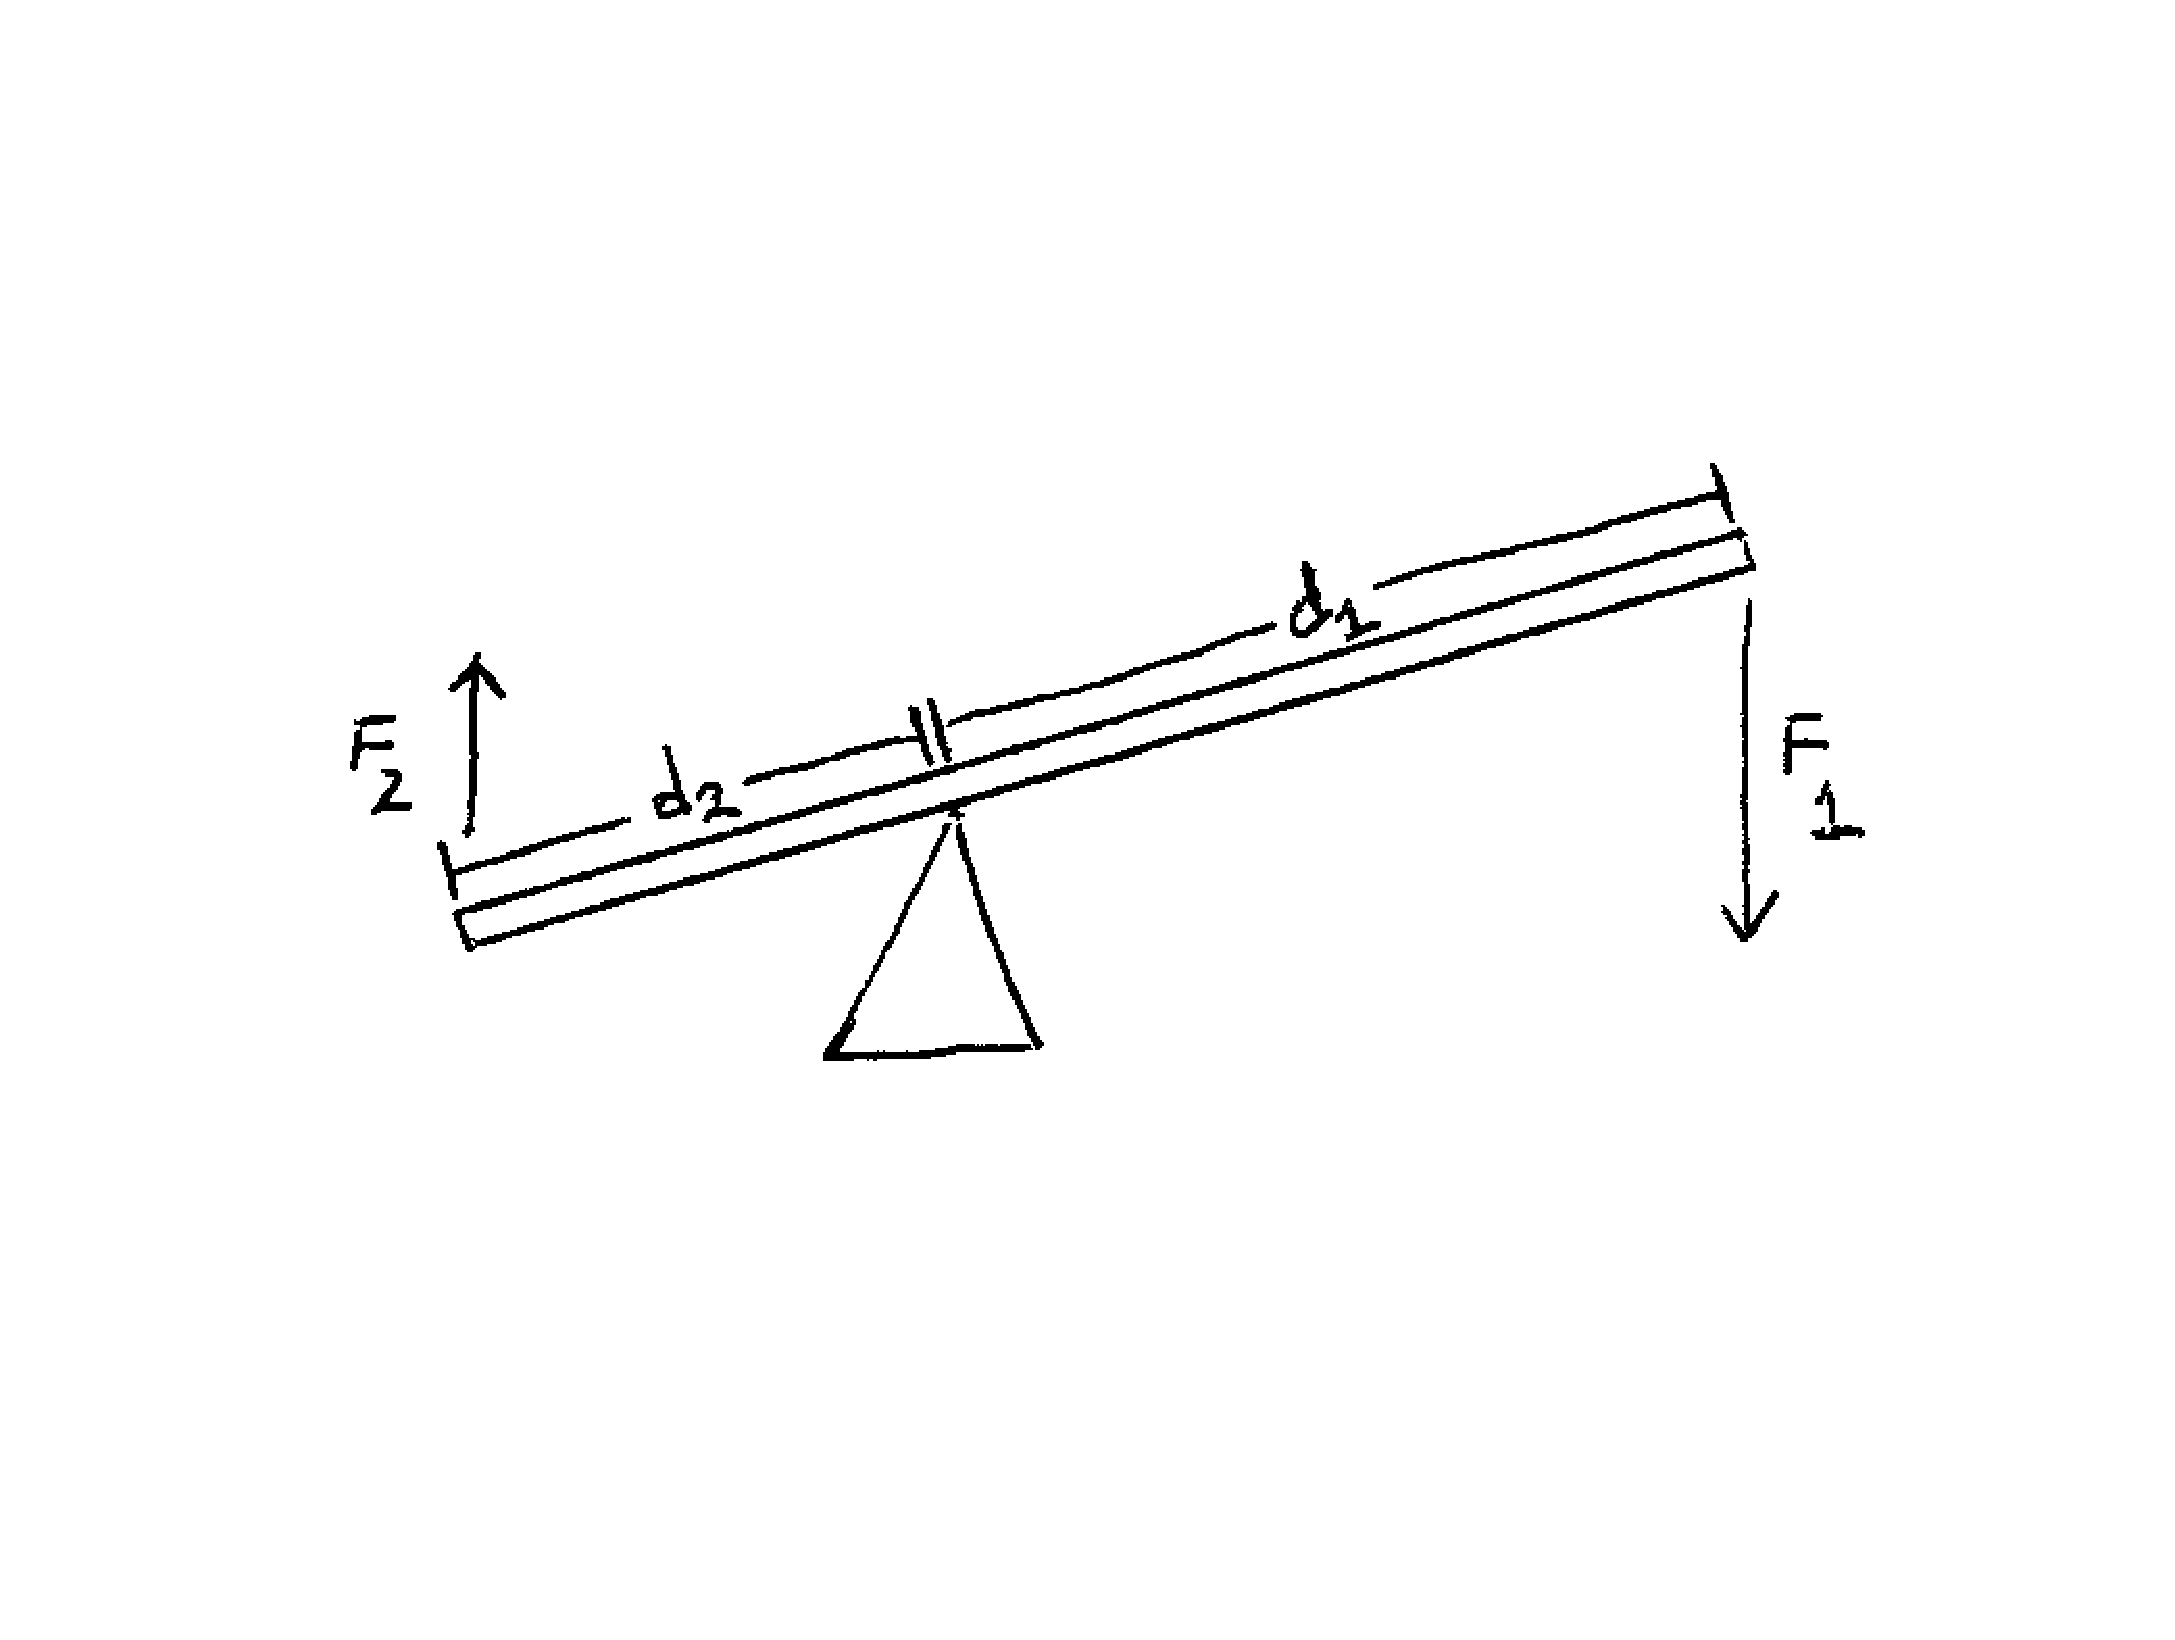
\includegraphics[width=0.5\textwidth]{images/lever.EPS}}
		\caption{A diagram of a lever.}
	\end{figure}

	\paragraph{Description}
	The lever provides a mechanical advantage the same way all simple mechanisms do: by translating distance into force. In the lever, a force $F_1$ exerted downward over distance $d_1$ is translated into a force $F_2$ over distance $d_2$. When distance $d_1$ is larger than distance $d_2$, less force is required to lift an object distance $d_2$, though it is over a longer distance. In this way levers maintain the amount of work done by reducing force and increasing distance.
		
	\subsection{The Wheel and Axle}
	
	\begin{figure}[H]
		\centerline{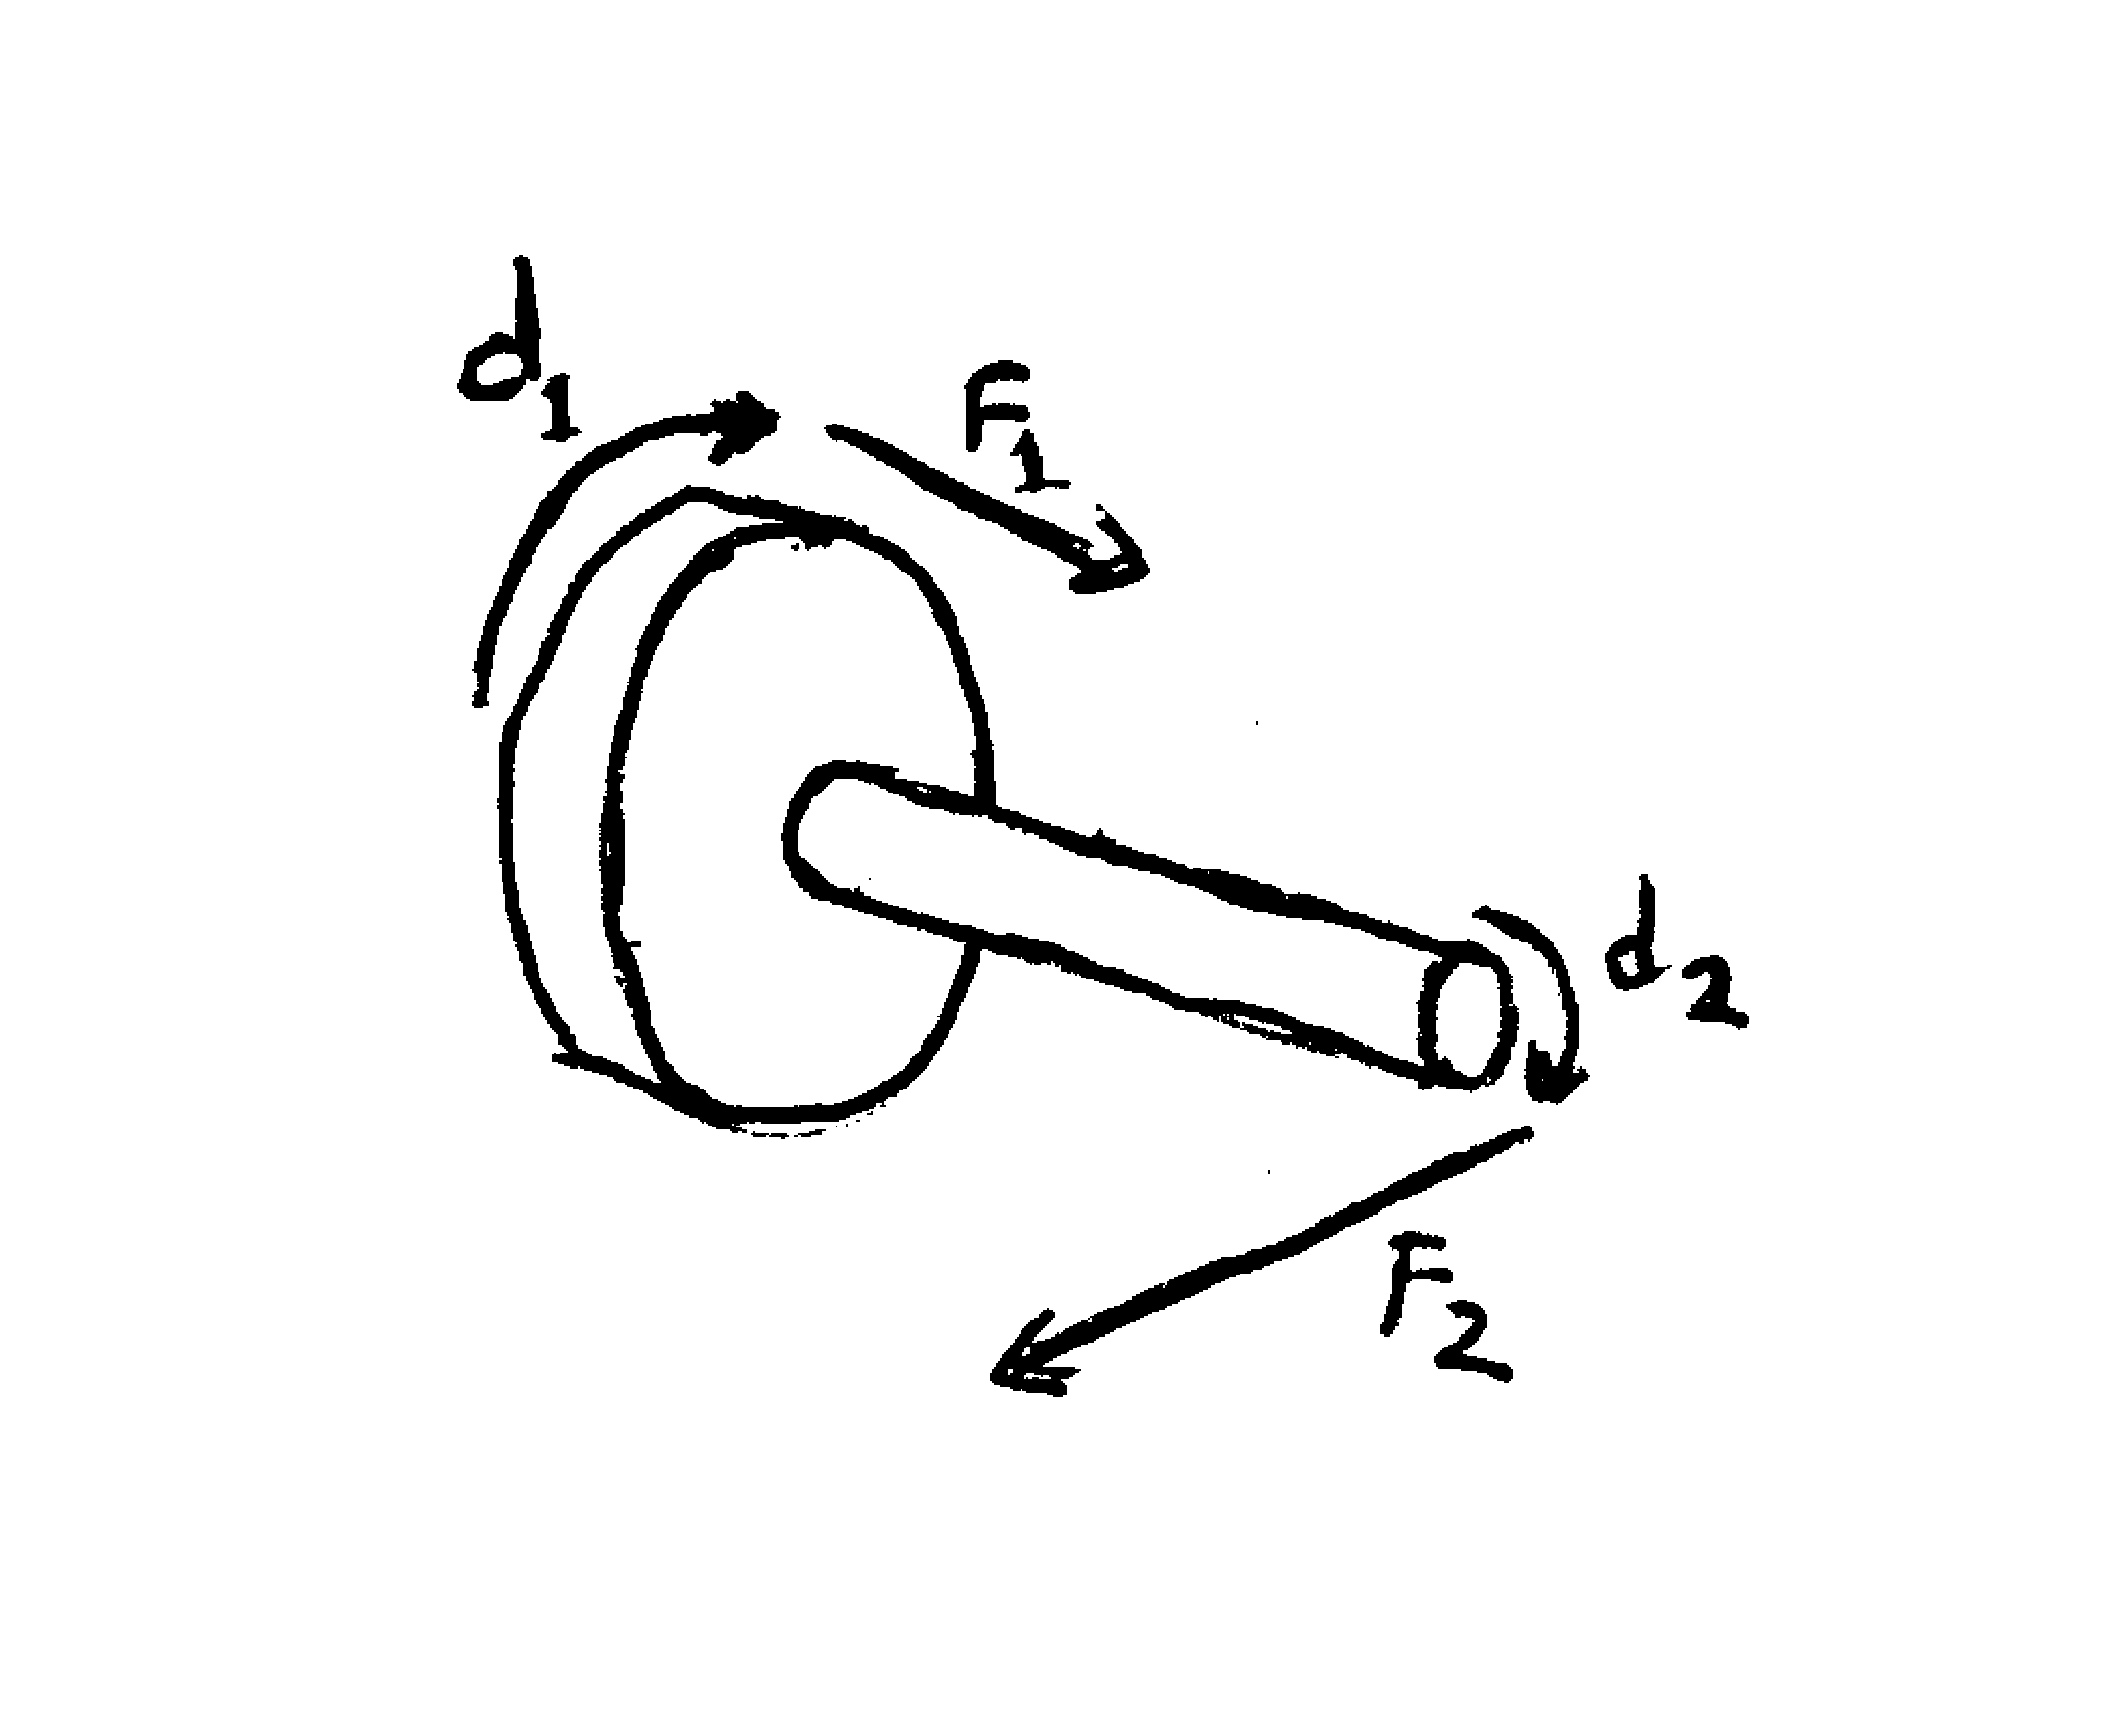
\includegraphics[width=0.5\textwidth]{images/wheel.EPS}}
		\caption{A diagram of a wheel and axle.}
	\end{figure}

	\paragraph{Description}
	The wheel and axle converts distance into force through the use of differently sized cylinders. Because the larger cylinder has to move a larger distance $d_1$ than the smaller cylinder's distance $d_2$, it's force must be smaller. Thus, when a force $F_1$ is applied on the larger cylinder over distance $d_1$, a larger force $F_2$ is applied on the smaller cylinder over a smaller distance $d_2$. In these diagrams the works on each "end" of the mechanism are equal, meaning $F_1 * d_1 = F_2 * d_2$. 
			
	\subsection{The Pulley}
	
	\begin{figure}[H]
		\centerline{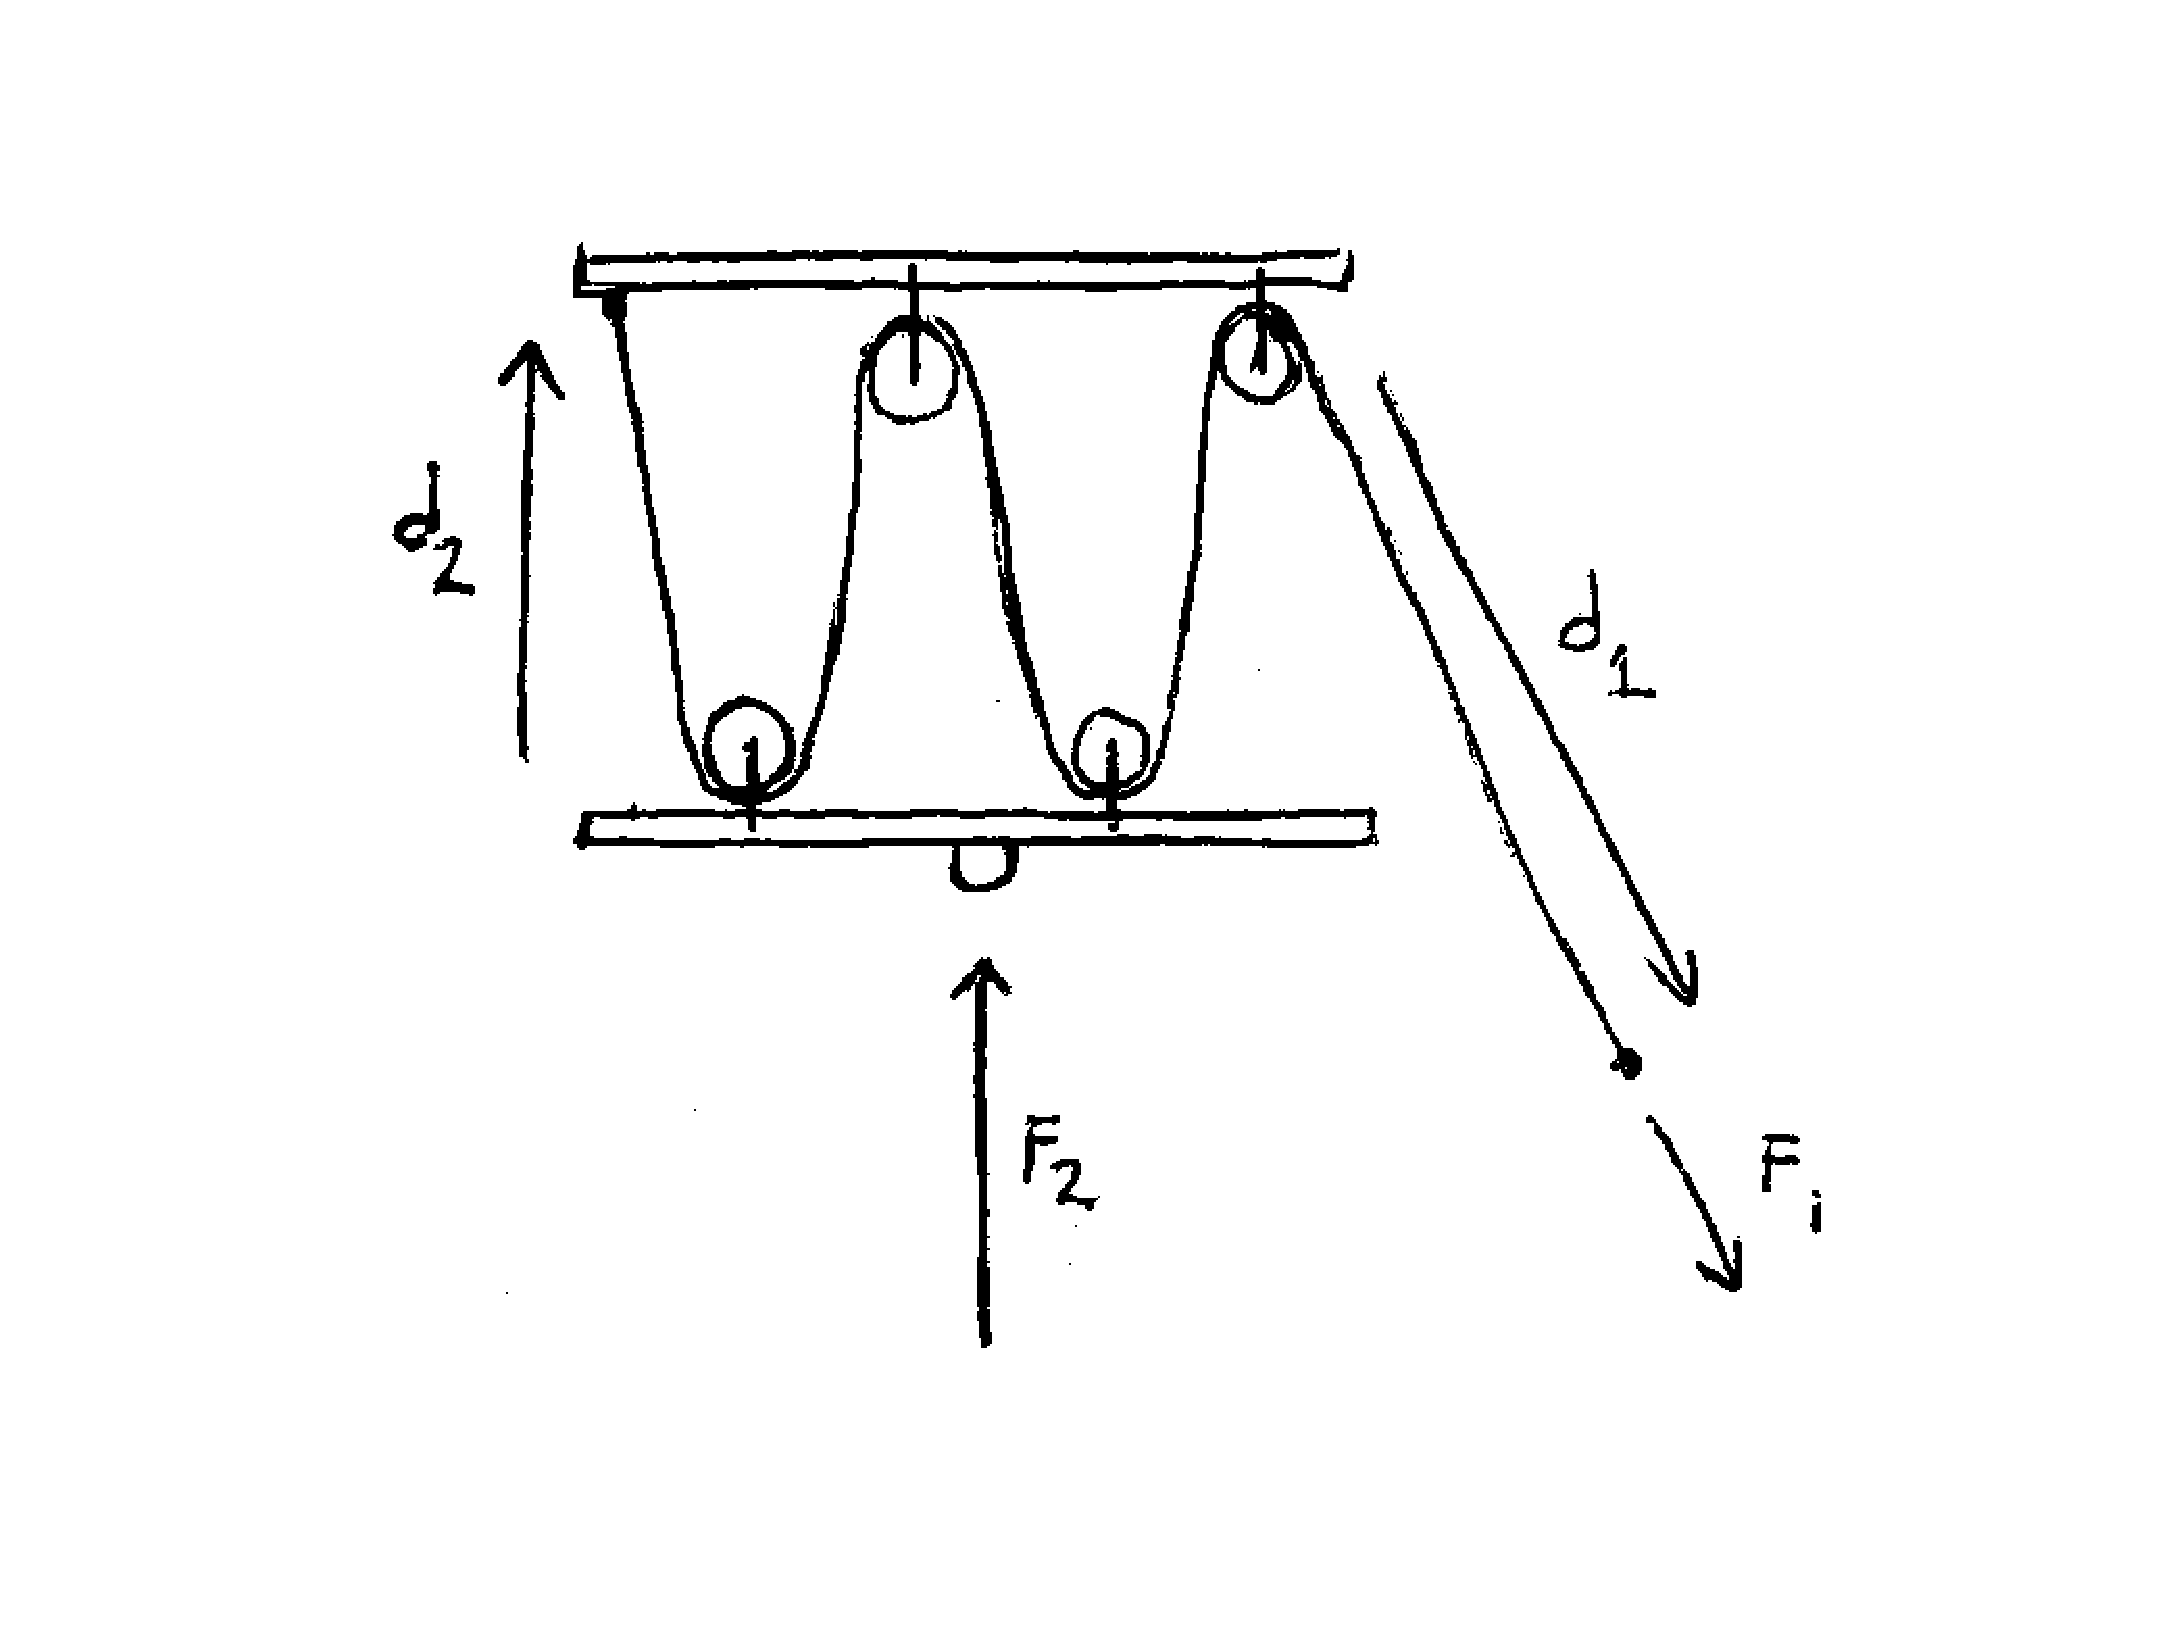
\includegraphics[width=0.5\textwidth]{images/pulley.EPS}}
		\caption{A diagram of a pulley.}
	\end{figure}

	\paragraph{Description}
	The pulley, or block and tackle, is often used to lift heavy objects with little force. As with all other simple mechanisms, this is achieved by increasing the distance over which a smaller force is exerted. The block and tackle does this by increasing the number of pulleys through which the rope passes between the top and the object. This means that to lift the object distance $d_2$, a distance of rope $d_1$ equal to $_2$ multiplied by the number of times the rope loops back and forth, minus one if the end of the rope goes down. For example, in this diagram $d_1$ is equal to $4 * d_2$, because the rope has four lengths connected to the bottom, excluding the one being directly pulled on. As with before, this increase in distance means a corresponding decreasing in force produces the same amount of work.
			
	\subsection{The Inclined Plane}
	\begin{figure}[H]
		\centerline{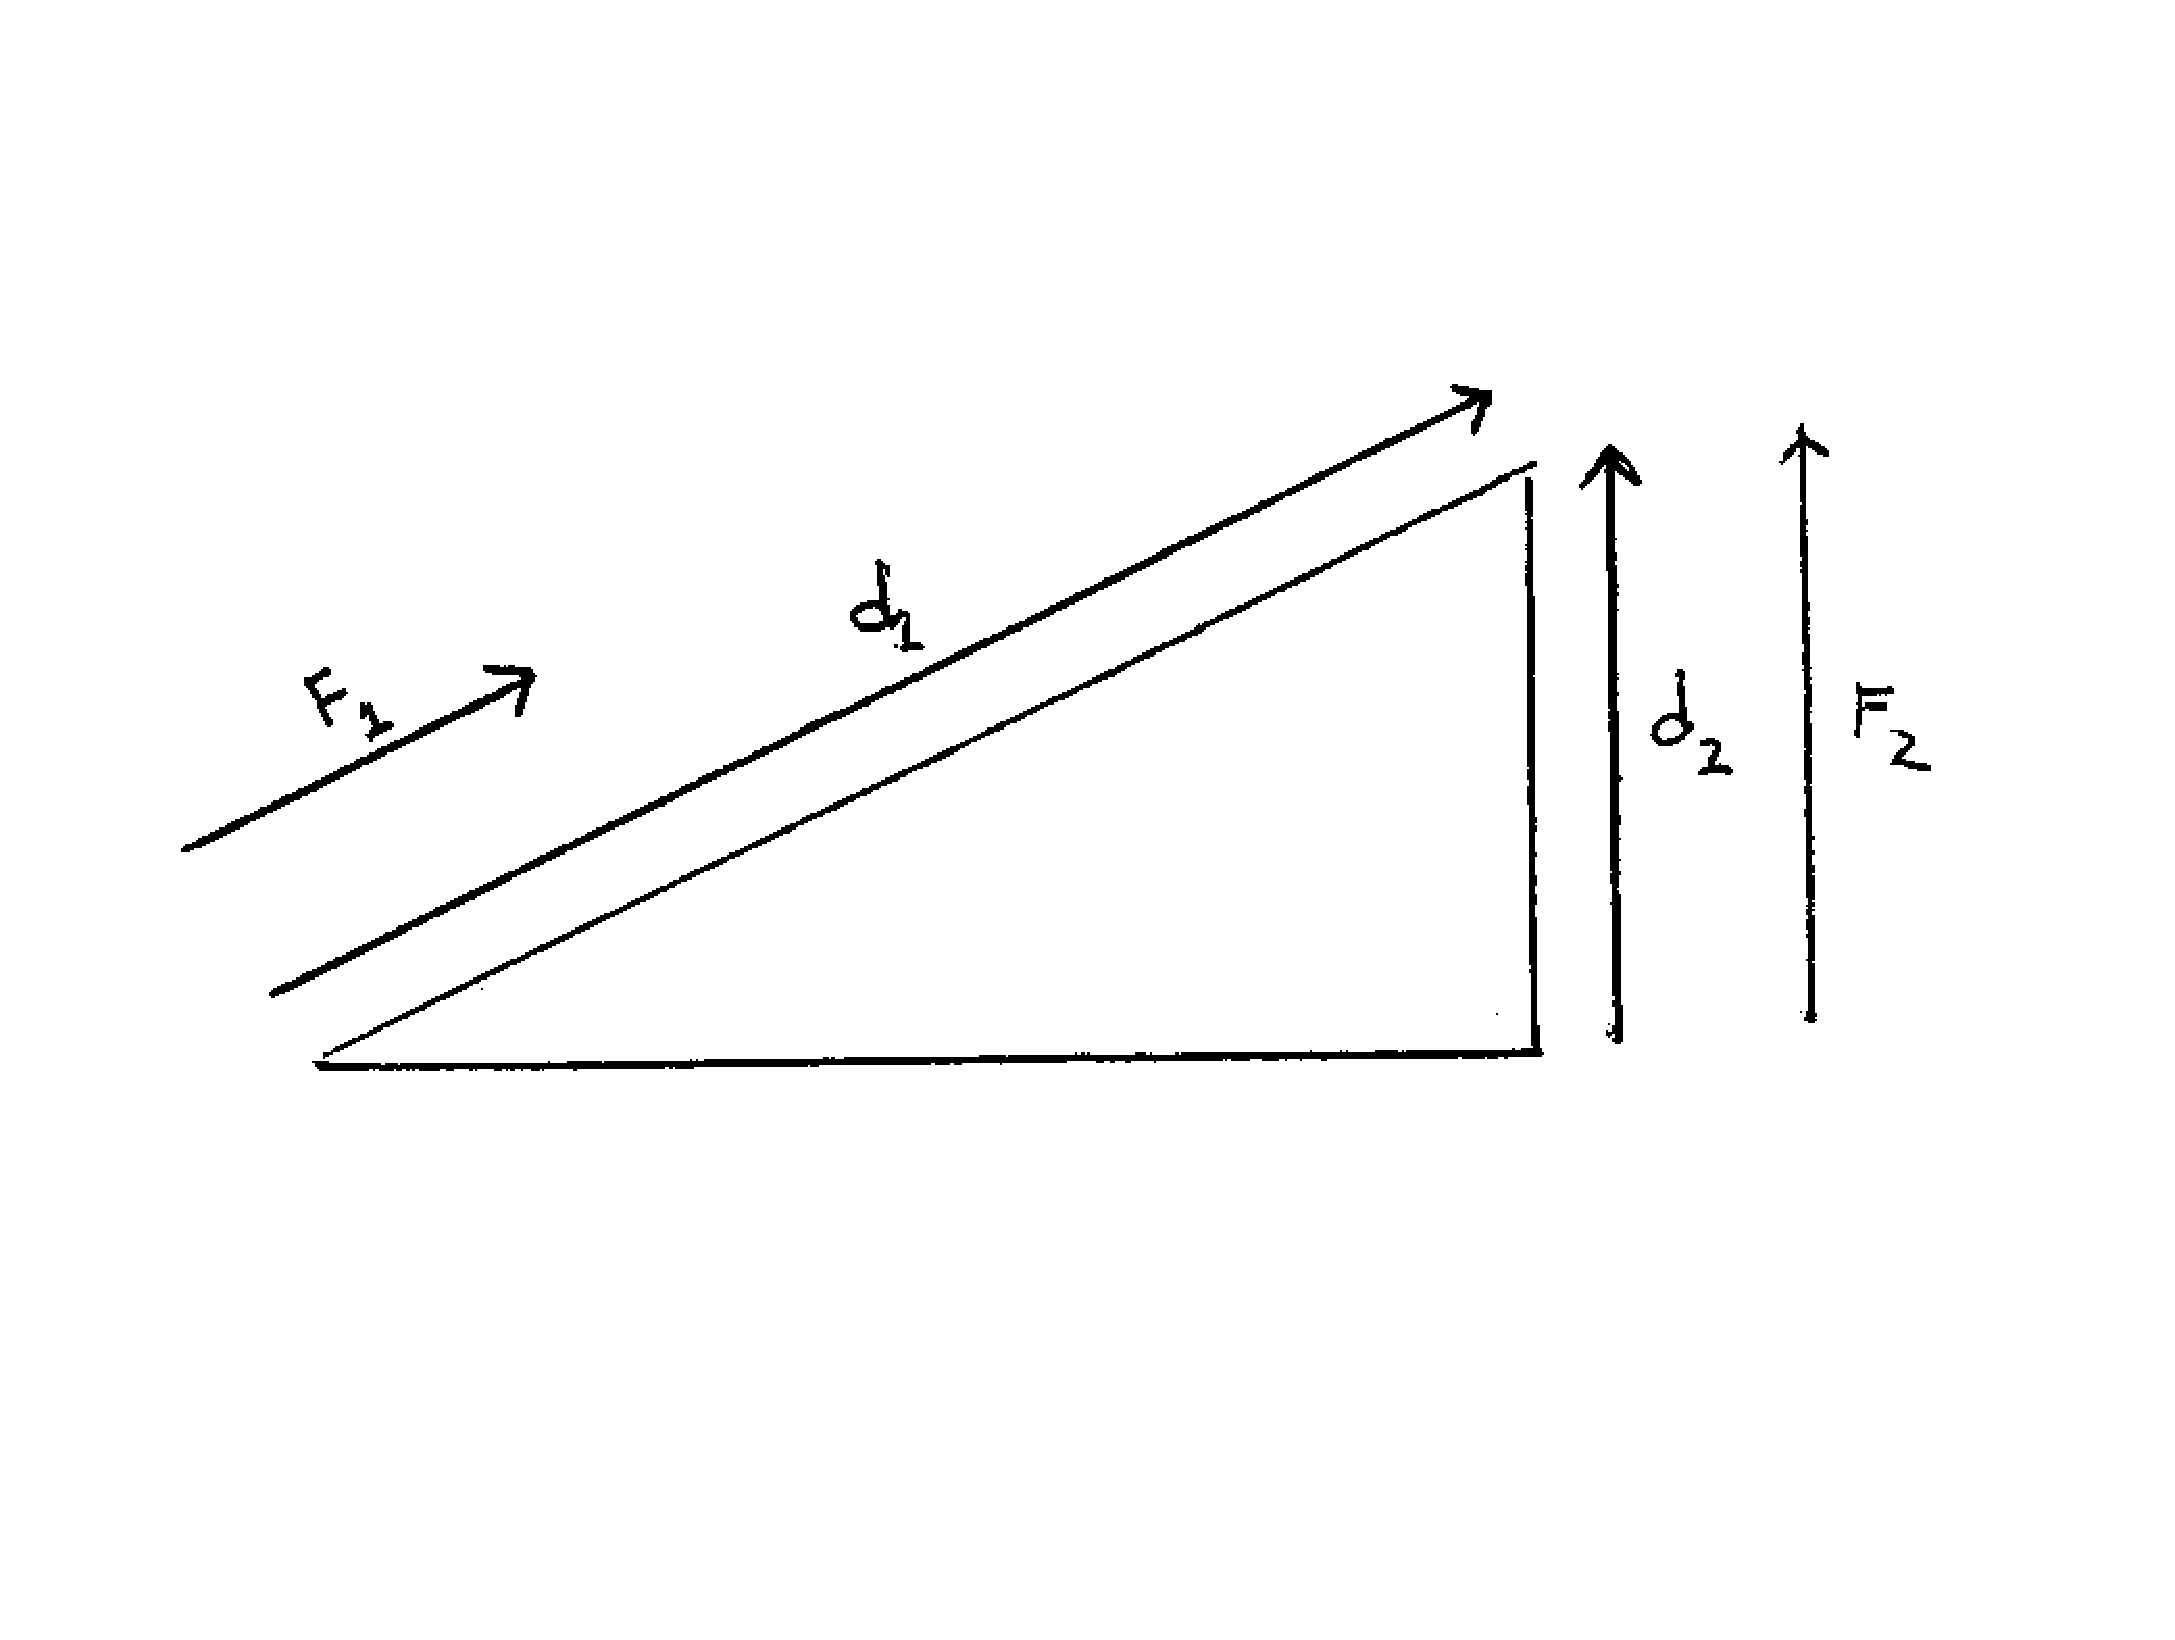
\includegraphics[width=0.5\textwidth]{images/plane.EPS}}
		\caption{A diagram of an inclined plane.}
	\end{figure}
	
	\paragraph{Description}
	Inclined planes are also often used to lift objects, but, unlike with pulleys, they decrease the amount of force necessary to lift an object a height $d_2$ by moving the object in a vertically diagonal line over a longer distance $d_1$. Similarly though, by increasing the distance $d_1$ they decrease the force $F_1$ required to do the same amount of work. This is immensely useful for simply moving heavy objects to a higher elevation, and is how roads going up hills work, extending the distance to decrease the force required of going straight up.
	
	\subsection{The Wedge}
	
	\begin{figure}[H]
		\centerline{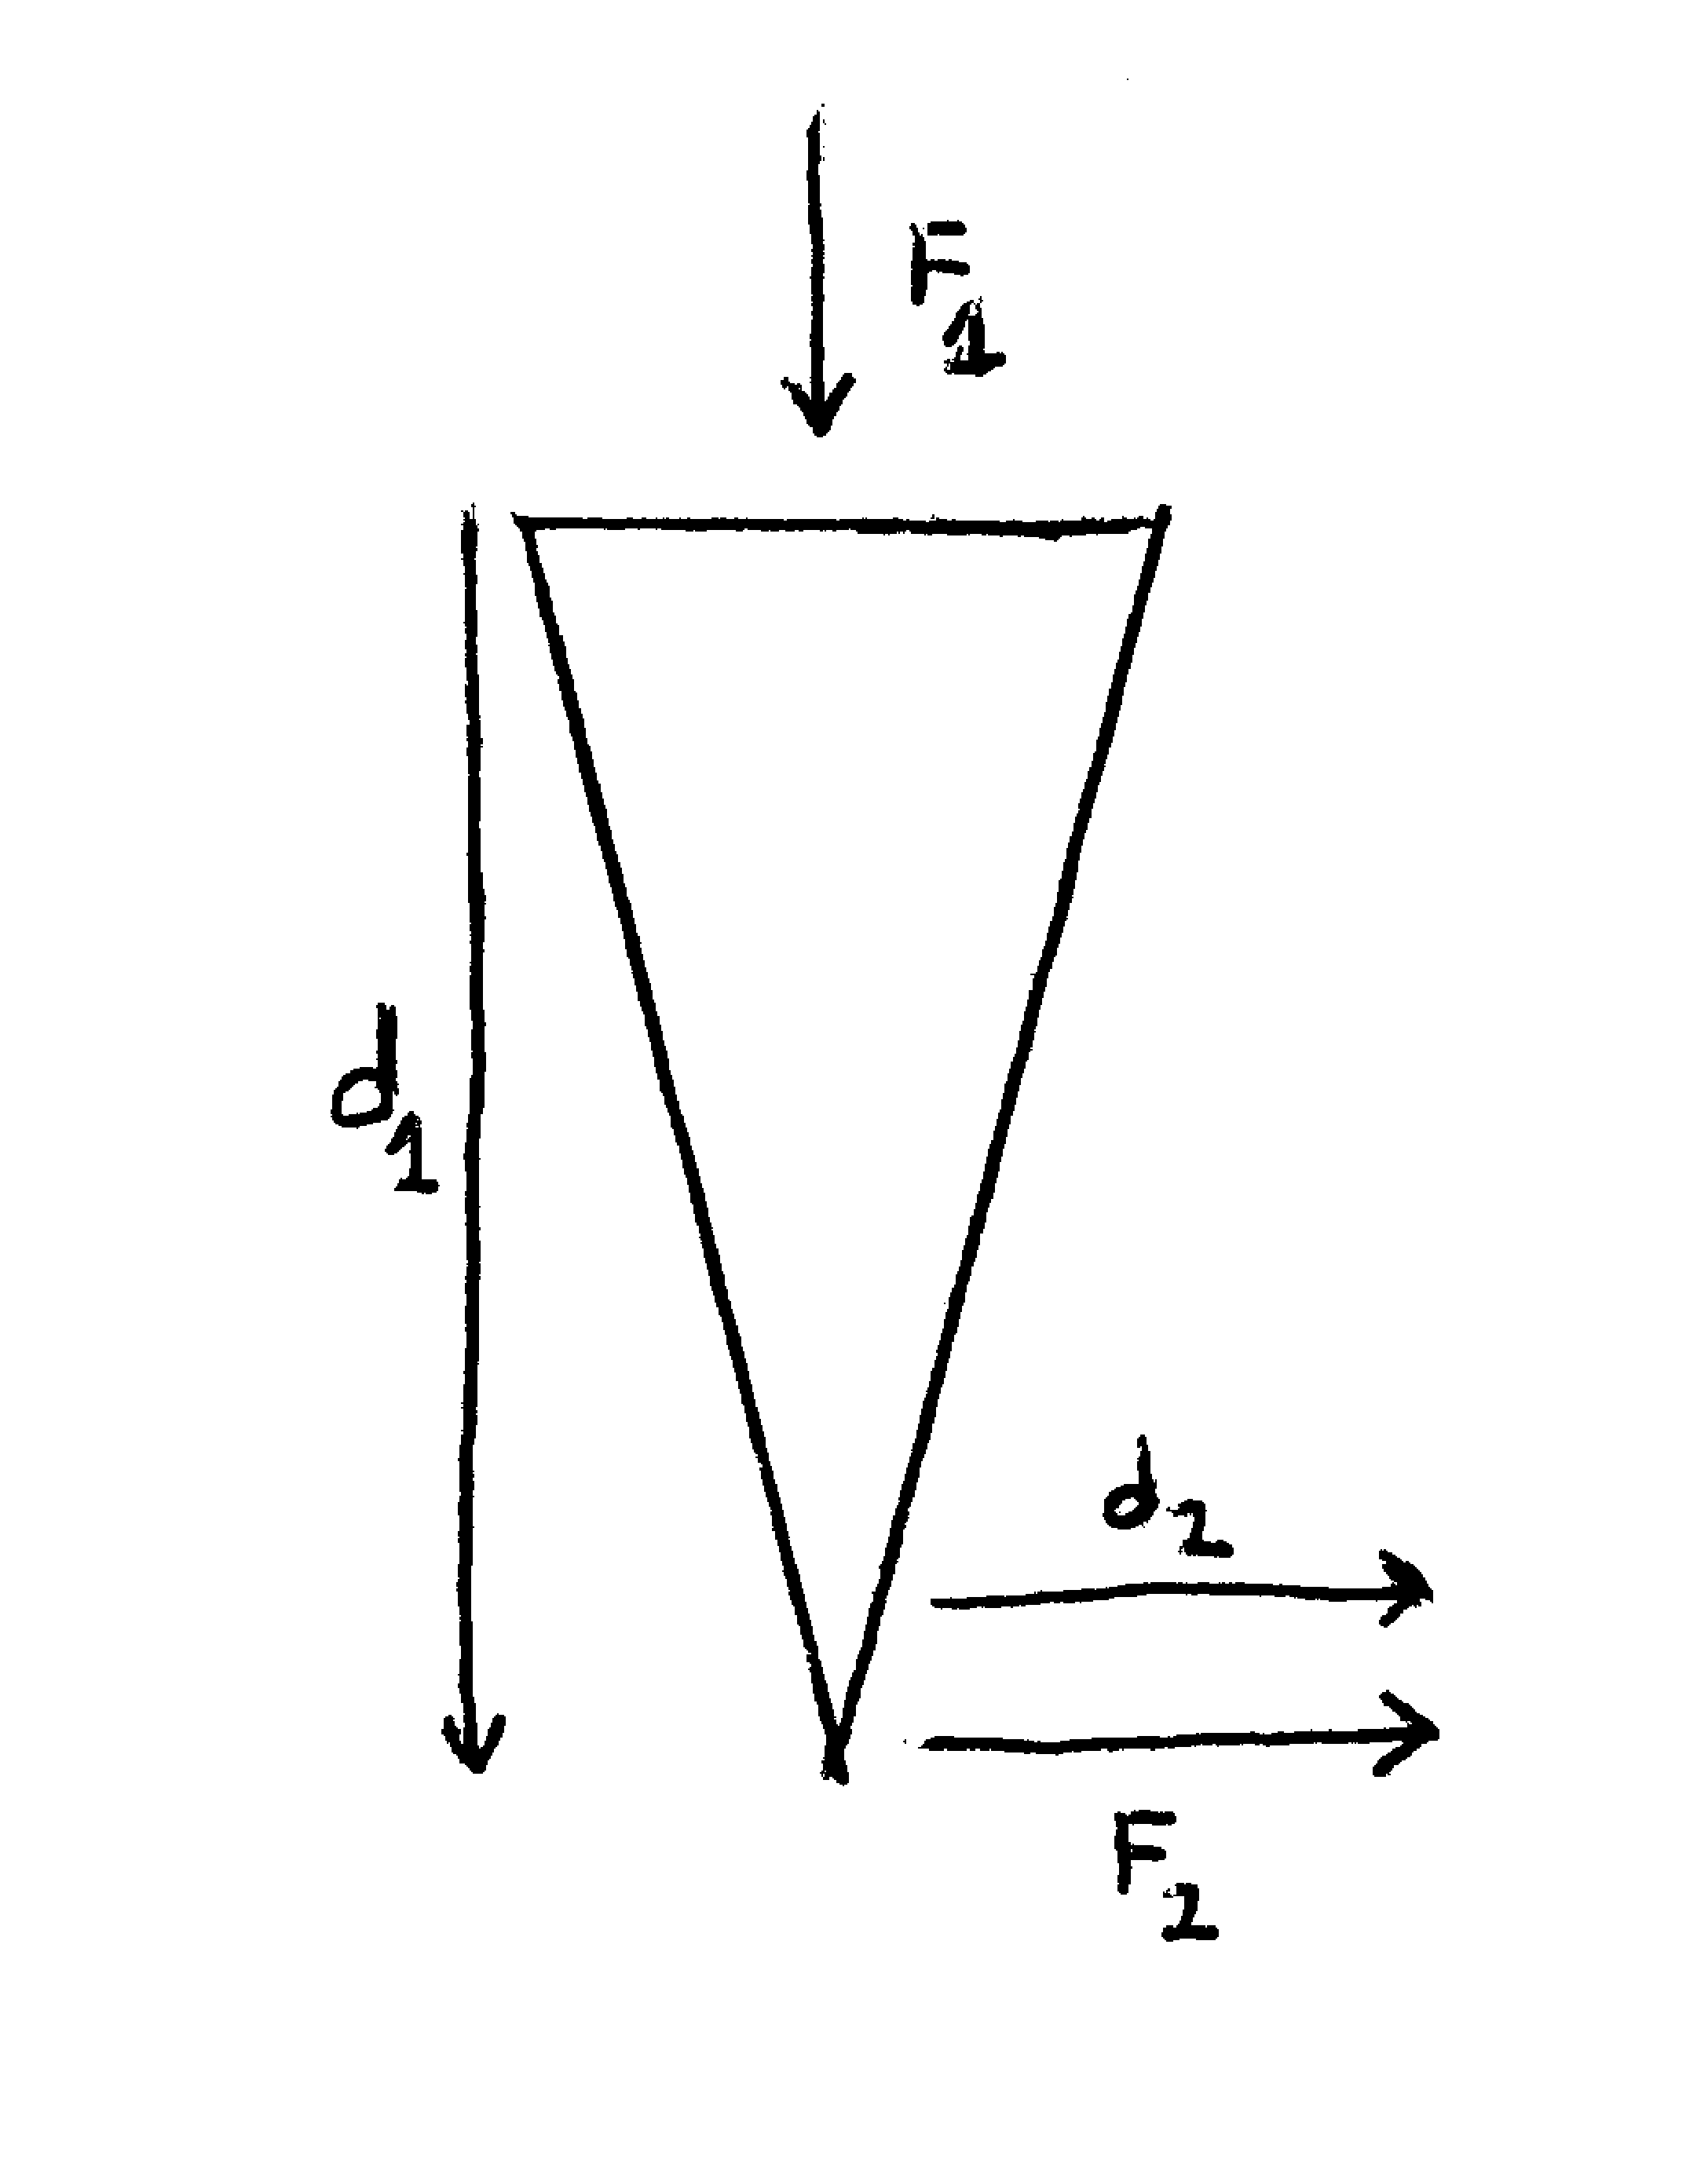
\includegraphics[width=0.5\textwidth]{images/wedge.EPS}}
		\caption{A diagram of a wedge.}
	\end{figure}

	\paragraph{Description}
	An extension of the inclined plane, the wedge uses the same principle of distributing work over larger distances to exert greater forces. This is often used to cut objects, both reducing the amount of force required, and increasing the force exerted. With a wedge, the downward force $F_1$ over distance $d_1$ exerts a larger force $F_2$ over a smaller distance $d_2$ on the surrounding material. Axes, knives, and many other common tools all use the principle of a wedge to make doing work easier and require less force.

	\subsection{The Screw}
	
	\begin{figure}[H]
		\centerline{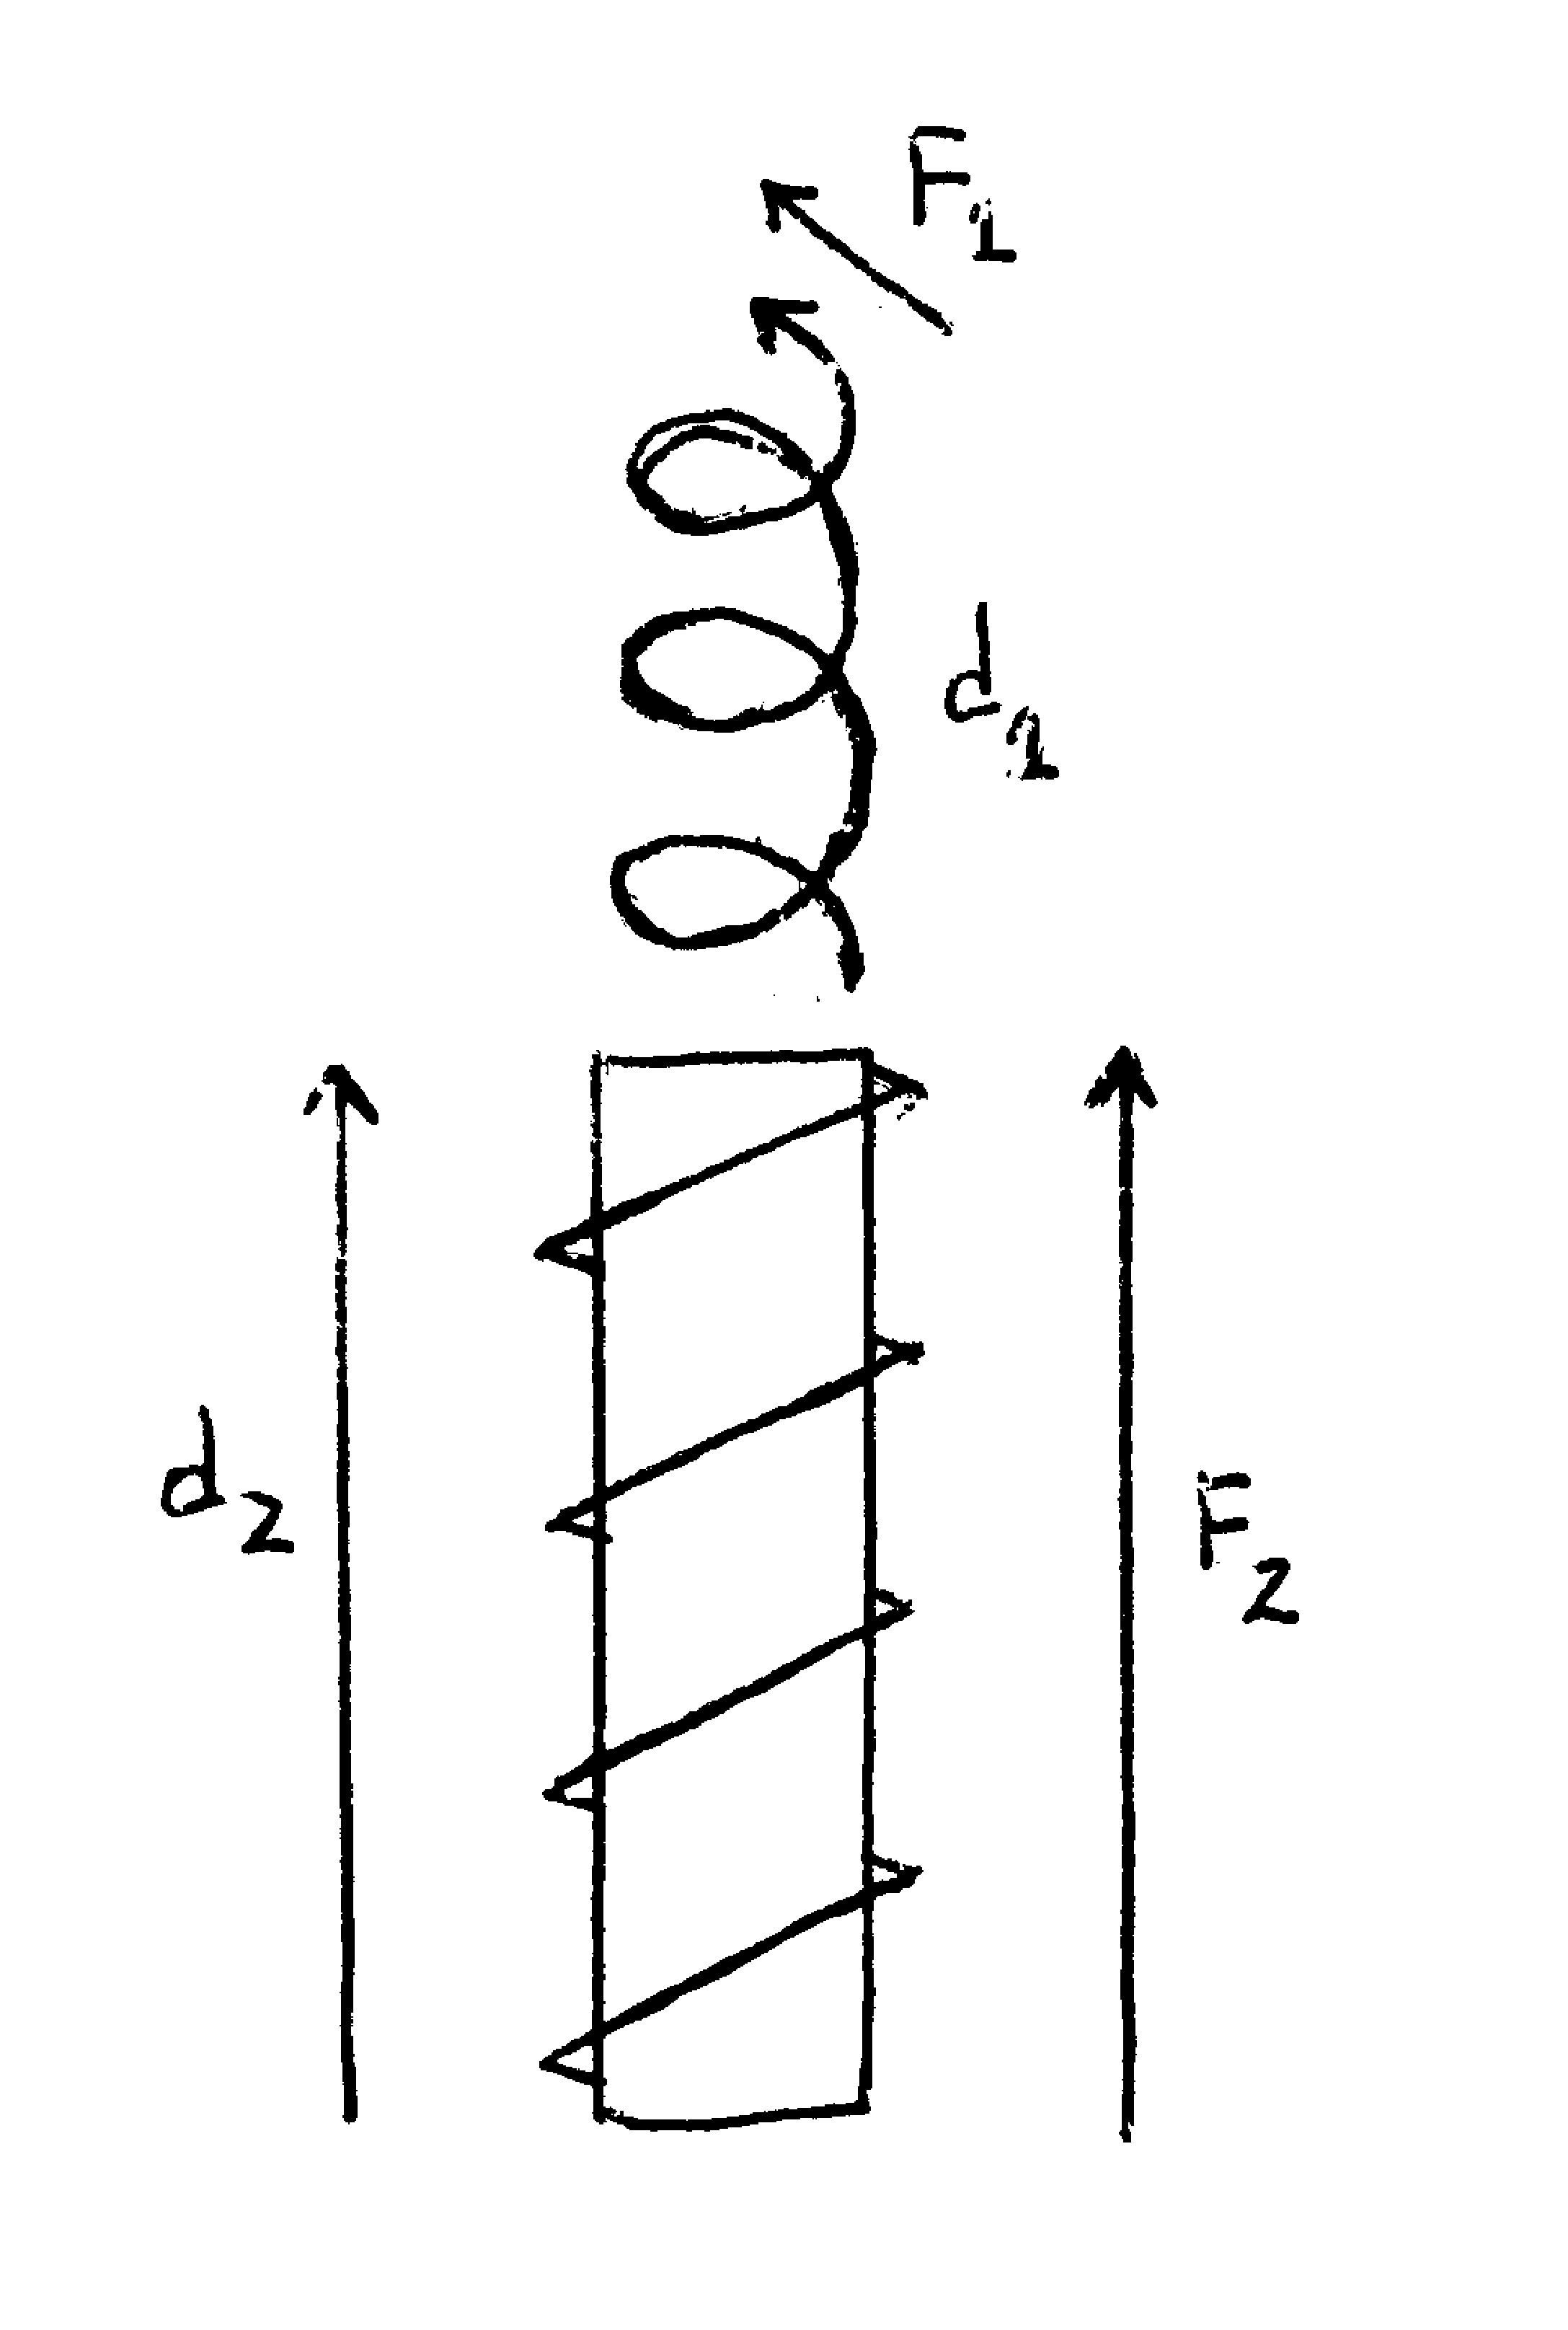
\includegraphics[width=0.5\textwidth]{images/screw.EPS}}
		\caption{A diagram of a screw.}
	\end{figure}
	
	\paragraph{Description}
	

	
	\section{Energy Storage}
	We have learned that energy can take a number of different forms. In this activity you will design and perform experiments to determine the amount of energy stored in several devices.

	\subsection{Mouse Trap}
	For this device, also estimate the velocity of the end of the bar when the trap is triggered.
	\paragraph{Experimental Design:}
	\paragraph{Data:}
	\paragraph{Calculations:}
	
	\subsection{Constant Acceleration Cars}
	For this device determine both the energy required to fully "charge" the car and the kinetic energy of the car when it is released. The percent efficiency of the device is the energy released divided by the energy required to charge it multiplied by 100.
	\paragraph{Experimental Design:}
	\paragraph{Data:}
	\paragraph{Calculations:}
	
	\subsection{Household Item}
	Experimentally determine the energy stored in the device and the device's efficiency.
	\paragraph{Experimental Design:}
	\paragraph{Data:}
	\paragraph{Calculations:}
	
	\subsection{Nerf Gun}
	Experimentally determine the work required to fully charge the Nerf Gun, the kinetic energy of the projectile, and the Nerf Gun's efficiency.
	\paragraph{Experimental Design:}
	\paragraph{Data:}
	\paragraph{Calculations:}
	
\end{document}
